\chapter{Loops}\label{CHAP_Loops}

\section{Difficulty: EASY}

\subsubsection*{Exercise 8.E01}
Using a {\code{WHILE}} loop, print the string {\code{"Hello World"}} 50 times.\\

\textit{Hints:
Don’t forget to include a counter in this {\code{WHILE}} loop.}\\[1cm]


% ------------------------------------------------------------------------------

\subsubsection*{Exercise 8.E02}
Copy the following list into your Jupyter Notebook:
\begin{figure}[H]
		\centering
		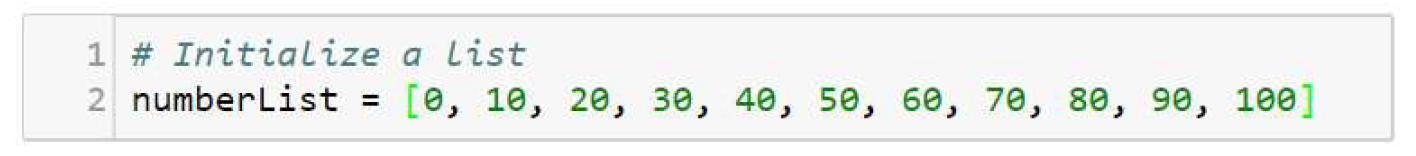
\includegraphics[width=\textwidth]{../IMG/8E02.png} 
\end{figure}
Using a {\code{FOR}} loop, print all the elements in the list.\\


\textit{Hints:
{\code{FOR}} loops don’t need a counter. The loop variable will automatically cycle through all elements in a sequence}\\[1cm]


% ------------------------------------------------------------------------------

\subsubsection*{Exercise 8.E03}
Using a {\code{WHILE}} loop, generate a list containing all the numbers between 0 and 1,000.\\


\textit{Hints:
You can solve this exercise with or without a counter. Remember: You can append new
elements to a list using the {\code{append()}} function. If you want to try the loop without the counter, remember you can determine the length of a list using the {\code{len()}} function.}\\[1cm]


% ------------------------------------------------------------------------------

\subsubsection*{Exercise 8.E04}
Using a {\code{WHILE}} loop, ask the user for their five favourite movies and store them in a list called {\code{favMovies}}.\\


\textit{Hints:
Use the {\code{input()}} function to request user input and the {\code{append()}} function to add new elements to a list.}\\[1cm]


% ------------------------------------------------------------------------------

\subsubsection*{Exercise 8.E05}
Using a {\code{WHILE}} loop, generate a list that stores the squares of all numbers between 0 and 1,000.\\


\textit{Hints:
You can calculate the square of a number using the ** operator.}\\[1cm]


% ------------------------------------------------------------------------------

\subsubsection*{Exercise 8.E06}
Copy the following list into your Jupyter Notebook:
\begin{figure}[H]
		\centering
		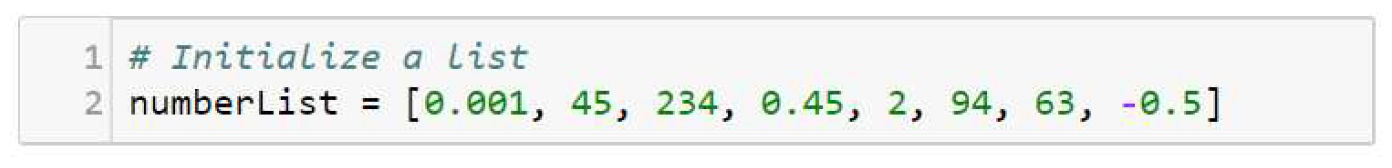
\includegraphics[width=\textwidth]{../IMG/8E06.png} 
\end{figure}
Using a {\code{FOR}} loop, generate a new list containing every object in the original list multiplied by 10.\\


\textit{Hints:
Use the * operator to perform a multiplication.}



% ------------------------------------------------------------------------------


\newpage
\section{Difficulty: MEDIUM}

\subsubsection*{Exercise 8.M01}
Using a {\code{WHILE}} loop, generate a list containing all the numbers between 1 and 10,000. Then, using another loop ({\code{WHILE}} or {\code{FOR}}) calculate the sum of all the numbers in the list.\\
Bonus:
Calculate the average of all the numbers in the list.\\


\textit{Hints:
You can use list indices to access specific objects in your list.}\\[1cm]


% ------------------------------------------------------------------------------

\subsubsection*{Exercise 8.M02}
Using a {\code{WHILE}} loop generate a list of all numbers between 0 and 1,000,000 that are a
multiple of 17. A number is a multiple of 17 if the modulus 17 of the number is equal to zero
meaning:
\begin{center}
	{\code{number \% 17 == 0}}
\end{center}
Determine how many objects are in the list.\\

\textit{Hints:
Insert an IF and ELSE statement inside your loop structure.}\\[1cm]


% ------------------------------------------------------------------------------

\subsubsection*{Exercise 8.M03}
Using the {\code{range()}} function and a {\code{FOR}} loop print all the numbers between 0 and 1,000.\\

\textit{Hints:
You can initialize the range instead of the usual sequence in the initialization line of your
{\code{FOR}} loop.}\\[1cm]


% ------------------------------------------------------------------------------

\subsubsection*{Exercise 8.M04 \red{[M]}}
Write a code that accepts a number $x$ from the user and calculates the factorial of $x$. The factorial $x!$ of $x$ is given by:
\begin{center}
$x! = x \cdot  (x-1) \cdot (x-2) \cdot ... \cdot 2 \cdot 1$.
\end{center}

\textit{Hints:
Your counter doesn't necessarily have to count up, it can also count down.}\\[1cm]


% ------------------------------------------------------------------------------

\subsubsection*{Exercise 8.M05}
Initialize a list containing all numbers between 1 and 20. Using a loop structure reverse the list.\\

\textit{Hints:
Store the reverse list in a new list and use the {\code{pop()}} function.}\\[1cm]


% ------------------------------------------------------------------------------

\subsubsection*{Exercise 8.M06}
Write a code that asks the user for a city and stores the city in a list. Continue asking the user for another city until the user enters the string {\code{STOP}} instead of a new city.\\


\textit{Hints:
You will need to check the input at every iteration step to test whether the {\code{STOP}} command has been entered. Use the {\code{BREAK}} command to forcefully exit a loop.}\\[1cm]


% ------------------------------------------------------------------------------

\subsubsection*{Exercise 8.M07}
Using a {\code{WHILE}} loop and the {\code{CONTINUE}} command, write a code that generates a list of all the numbers between 0 and 1,000 but do not include any numbers that are divisible by 5. Count the number of elements in your list once you’re done.\\


\textit{Hints:
To check whether a number is divisible by 5, check whether the modulus 5 is equal to zero. If
{\code{num \% 5 == 0}} then the number is divisible by 5.}\\[1cm]


% ------------------------------------------------------------------------------

\subsubsection*{Exercise 8.M08}
In this exercise you will pick a number $x$ and allow the user to guess the number.
\begin{enumerate}[label=(\alph*)]
	\item Set $x$ to a number between 0 and 10. The user is allowed to guess three times. If the user guesses the number, the user wins. If the user fails to guess the number after
three tries, the computer wins. Display a message declaring the winner.
	\item Set $x$ to a number between 0 and 1,000. Allow the user to guess until they have
guessed the number correctly. Whenever the user enters a wrong number, tell them
whether the actual number is smaller or larger than the guess. Keep track of how
many guesses it took the user to get to the right number.
\end{enumerate}

\textit{Hints:
Remember you need to convert the user input from a string to an integer using the int()
function to perform mathematical operations on it. You will need {\code{IF and ELSE}}
statements inside your loop (maybe even nested {\code{IF and ELSE}} statements).}\\[1cm]


% ------------------------------------------------------------------------------

\subsubsection*{Exercise 8.M09 \red{[M]}}
A prime number is an integer that can be divided without a remainder only by 1 or itself.
\begin{enumerate}[label=(\alph*)]
	\item Write a code that stores all prime numbers between 1 and 1000 in a list. (Note: 1 is not a prime number!)
	\item Count the number of prime numbers between 1 and 1000 without using the len()
function.
\end{enumerate}

\textit{Hints:
You can check all prime numbers between 2 and 10,4729 here:
\url{https://primes.utm.edu/lists/small/10000.txt}. You will need a nested loop and {\code{IF and ELSE}} statements.}\\[1cm]


% ------------------------------------------------------------------------------

\subsubsection*{Exercise 8.M10}
Ask the user to enter a three-digit pin code containing numbers between 0 and 9. The write
a code that guesses the pin code.\\


Hints:
You will three nested loops each with their own counter, the {\code{BREAK}} and the {\code{CONTINUE}} command. Remember: To convert strings into integers use the {\code{int()}} function, to convert integers into strings use the {\code{str()}} function.\\[1cm]


% ------------------------------------------------------------------------------

\subsubsection*{Exercise 8.M11}
You have ten students in your class:\\
Oliver, Harry, George, Jack, Jacob, Olivia, Amelia, Emily, Isla, and Ava.\\
You ask them to pair up for an exercise. Using nested loops, find all possible group
constellations. Count the total number of constellations.\\


\textit{Hints:
You will need nested loops with their own individual counters here. Remember that you
can’t pair students with themselves so you will also need an {\code{IF and ELSE}} statement
structure to take care of those cases.}\\[1cm]


% ------------------------------------------------------------------------------

\subsubsection*{Exercise 8.M12 \red{[M]}}
The number $\pi$ is a mathematical constant you can access via python libraries. You can also
calculate it using the Leibniz formula:\\
\begin{center}
	$\frac{\pi}{4} = \sum_{k=0}^{n} \frac{(-1)^k}{2\cdot k+1}|_{n\rightarrow \infty}$.
\end{center}
We cannot solve this equation for all values of $k$, but by choosing a large enough $n$ when can approximate the value of $\pi$ using a loop over $k$ for the summation:
\begin{center}
	$\pi \approx 4 \cdot \sum_{k=0}^{n} \frac{(-1)^k}{2\cdot k+1}$.
\end{center}
Write a code that approximates $\pi$ for
\begin{enumerate}[label=(\alph*)]
	\item $n = 10$
	\item $ = 100$
	\item $ = 1000$
\end{enumerate}
and calculate how much the obtain values deviate from the {\code{math.pi}} value.\\


\textit{Hints:
To use the {\code{math}} library you need to import it first using {\code{import math}}.}\\[1cm]


% ------------------------------------------------------------------------------

\subsubsection*{Exercise 8.M13}
Generate two lists:
\begin{center}
	{\code{L1 = [1, 2, 3, 4, 5, 6, 7, 8, 9, 10]}}
\end{center}
and
\begin{center}
	{\code{L2 = [8, 9, 10, 11, 12, 13]}}
\end{center}
and write a code that
\begin{enumerate}[label=(\alph*)]
	\item compares both lists and returns a new list containing elements that are present in
both {\code{L1}} and {\code{L2}}.
	\item  compares both lists and returns a new list containing elements that are present in
either {\code{L1}} or {\code{L2}} but not in both.
\end{enumerate}

\textit{Hints:
You can test whether an object is in a list using the {\code{in}} function.}\\[1cm]


% ------------------------------------------------------------------------------

\subsubsection*{Exercise 8.M14}
Write a code that accepts two strings from the user. Check whether the two strings are
anagrams of each other. Display the result.\\
{\code{string1}} and {\code{string2}} are anagrams if {\code{string1}} can be turned into {\code{string2}} simply by reshuffling the letters in it. For example: drawer and reward are anagrams.\\


\textit{Hints:
You can check your code with this website: \url{https://www.wordplays.com/anagram-solver/}.}\\[1cm]


% ------------------------------------------------------------------------------

\subsubsection*{Exercise 8.S01}
Write a code that finds the longest string in a string list of arbitrary length.\\


\textit{Hints:
You can find the length of a list using the len() function or use a FOR loop to iterate over all elements in a list. You can generate random words here: \url{https://www.randomlists.com/random-words} to test your code.}\\[1cm]


% ------------------------------------------------------------------------------

\subsubsection*{Exercise 8.S02}
Remember Armstrong numbers from exercise 6.H01:\\
An Armstrong number (also known as narcissistic number) is a number that is the sum of its
own digits each raised to the power of the digit number.\\
For example: $153 \rightarrow 1^3 + 5^3 + 3^3 = 1 + 125 + 27 = 153$\\
Instead of writing a code that tests whether a 3-digit number is an Armstrong number as we
did in 6.H01, write a code that take a number of arbitrary length and determine whether it is
an Armstrong number.\\


\textit{Hints:
You can check your code using this website: \url{http://mathworld.wolfram.com/NarcissisticNumber.html}.}



% ------------------------------------------------------------------------------

\newpage
\section{Difficulty: HARD}

\subsubsection*{Exercise 8.H01}
Generate a two-dimensional list with each element of the parent list containing a child list
which in turn contains two elements: The name of a costumer and their mobile phone
number. For example:\\
\begin{center}
	{\code{costumer = [[“Donald Duck”, “123456789”], [“Mickey Mouse”, “987654321”], ...]}}
\end{center}
Write a code that asks the user for the name of a costumer. If the name is not in the list,
print an error message. If the name is in the list, return the corresponding mobile phone
number.\\


\textit{Hints:
When you’re working with nested lists, remember that each child list will correspond to an
additional index. Sometimes it helps drawing the list structure on a piece of paper.}\\[1cm]


% ------------------------------------------------------------------------------

\subsubsection*{Exercise 8.H02 \red{[M]}}
There are multiple ways to express numbers. The most common one is the decimal number
system (base 10) which we use in our everyday life. Computers on the other hand tend to
use a binary system (base 2) in which numbers are represented by combinations of the digits
0 and 1. In this exercise you will
\begin{enumerate}[label=(\alph*)]
	\item Write a code that converts any decimal integer provided by the user
into a binary number
	\item Write a code that converts any binary number provided by the user and
converts it into a decimal integer
\end{enumerate}
Below you can find an explanation and worked examples on how the conversions work. Visit
\url{http://calc.50x.eu/} to check whether your code works.\\

\textbf{Converting a Decimal Number into a Binary:}
To convert a decimal number $x$ into a binary perform the following steps:
\begin{enumerate}
	\item Divide $x$ by 2
	\item Take note of the remainder $x\%2$ (which will be either 0 or 1)
	\item Set $x$ equal to the result of the division: $x = x/2$
	\item Repeat step 1-4 until $x = 0$
	\item Reverse the order of the remainders
\end{enumerate}
Example:\\
Let’s convert the number $108_2$ into a binary:
\begin{figure}[H]
		\centering
		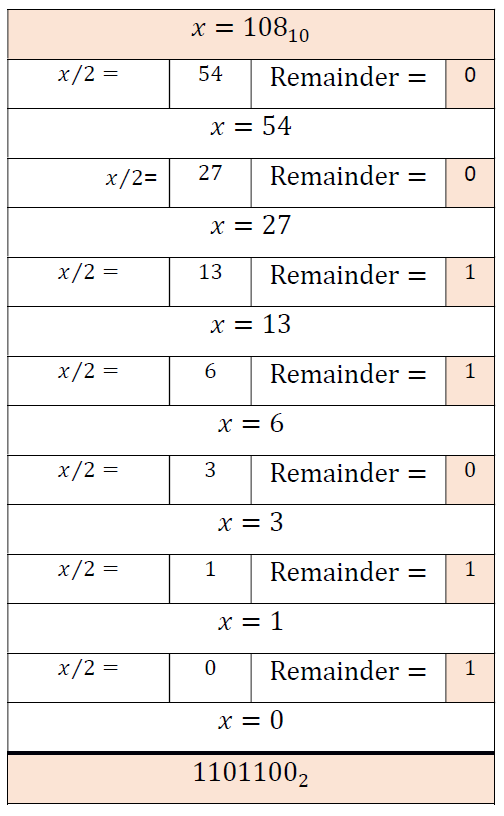
\includegraphics[width=0.4\textwidth]{../IMG/8H02_1.png} 
\end{figure}

\textbf{Converting a Binary Number into a Decimal:}
To convert a binary number $b$ into a decimal perform the following steps:
\begin{enumerate}
	\item Write down the binary number
	\item Underneath each binary digit note down the powers of two going from right to left
	\item Multiply each binary digit with its corresponding power of two
	\item Add the power of two values together
\end{enumerate}
Example:\\
Let’s convert the number $1101100_2$ back into a decimal:
\begin{figure}[H]
		\centering
		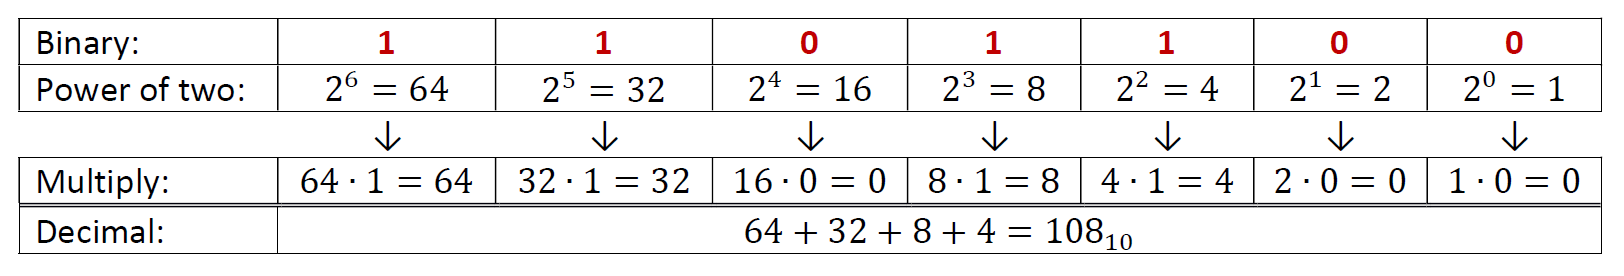
\includegraphics[width=\textwidth]{../IMG/8H02_2.png} 
\end{figure}

\textit{Hints:
You will need the modulus operator \%, the floor division operator //, the exponent operator **, and eventually you will want to reverse a string which can be done via {\code{str[::-1]}}.}\\[1cm]


% ------------------------------------------------------------------------------

\subsubsection*{Exercise 8.H03 \red{[M]}}
In this exercise you will be writing a code to perform matrix additions and multiplications.
A matrix is a mathematical construct with numbers arranged in columns ($c$) and rows ($r$). The simplest example is the vector with 1 column and an arbitrary number of rows ($1 \times r$), this is called a vector.\\
In this exercise however, we will be looking at larger matrices. For these objects, addition
and multiplication are bit a bit more complex. Below you can find the addition and
multiplication rules for ($n \times n$) matrices:\\


\textbf{Matrix-Number Multiplication:}
\[
4 \cdot
  \begin{bmatrix}
    5 & 6\\
    7 & 8
  \end{bmatrix} = 
  \begin{bmatrix}
    4 \cdot 5 & 4 \cdot 6\\
    4 \cdot 7 & 4 \cdot 8
  \end{bmatrix} =
  \begin{bmatrix}
    20 & 24\\
    28 & 32
  \end{bmatrix}
\]

\textbf{Matrix Addition:}
\[
  \begin{bmatrix}
    1 & 2\\
    3 & 4
  \end{bmatrix} +
  \begin{bmatrix}
    5 & 6\\
    7 & 8
  \end{bmatrix} =
  \begin{bmatrix}
    1+5 & 2+6\\
    3+7 & 4+8
  \end{bmatrix} =
  \begin{bmatrix}
    6 & 8\\
    10 & 12
  \end{bmatrix}
\]

\textbf{Matrix-Matrix Multiplication:}
\[
  \begin{bmatrix}
    1 & 2\\
    3 & 4
  \end{bmatrix} \times
  \begin{bmatrix}
    5 & 6\\
    7 & 8
  \end{bmatrix} =
  \begin{bmatrix}
    1 \cdot 5 + 2 \cdot 7 & 1 \cdot 6 + 2 \cdot 8\\
    3 \cdot 5 + 4 \cdot 7 & 3 \cdot 6 + 4 \cdot 8
  \end{bmatrix} =
  \begin{bmatrix}
    19 & 22\\
    43 & 50
  \end{bmatrix}
\]



Write a code that
\begin{enumerate}[label=(\alph*)]
	\item multiplies a ($c \times r$) matrix by a number.
	\item calculates the sum of two matrices. Start with the simple $(2 \times 2) \times (2 \times 2)$ case as shown in the examples above. Then extend it to the more general case of $(n \times n) \times (n \times n)$.
	\item calculates the product of two matrices. Start with the simple $(2 \times 2) \times (2 \times 2)$ case as shown in the examples above. Then extend it to the more general case of $(n \times n) \times (n \times n)$.
\end{enumerate}


\textit{Hints:
To help you visualize larger matrices, I have included a python script called\\
{\code{matrixOperations.py}}. It's in the same directory as the solution to this exercise. Place the file in the same folder as your Jupyter Notebook or script. The add {\code{from matrix\_operations import matrixPrint}} to the top of your script. You can now use (a very basic) matrices visualization routine by typing {\code{matrixPrint(matrixName)}}.}